% ============================================================
% DS MOD08 -- Loi normale : réglage, cumul de durées, décision (corrigé et barème)
% BTS ATI / CRSA -- durée 1 h -- document formateur
% Pôle Formation UIMM - CVDL - S. JAUBERT
% Sujet : MOD08_DS_Loi_Normale_ATI_CRSA_v1_0
% Références : TD MOD08 v2.0 (dossier remis aux stagiaires), problème, question, page imprimée
% ============================================================
\documentclass[a4paper,11pt]{article}
\usepackage[utf8]{inputenc}
\usepackage[T1]{fontenc}
% babel-french absent sur certains postes : chargement conditionnel
\IfFileExists{french.ldf}{\usepackage[french]{babel}}{}
\usepackage{helvet}
\usepackage{courier}
\renewcommand{\familydefault}{\sfdefault}
\usepackage[top=3cm, bottom=2.5cm, left=2cm, right=2cm, headheight=2cm]{geometry}
\usepackage{amsmath,amssymb,amsfonts}
\usepackage{graphicx}
\usepackage[dvipsnames,table]{xcolor}
\usepackage{tikz}
\usepackage[most]{tcolorbox}
\usepackage{fancyhdr}
\usepackage{enumitem}
\usepackage{array,needspace,booktabs}
\usepackage{titlesec}
\usepackage{hyperref}

\definecolor{uimmblue}{HTML}{005C85}
\definecolor{uimmred}{HTML}{D31326}
\definecolor{uimmlightblue}{HTML}{E8F1F8}
\definecolor{uimmgray}{HTML}{333333}
\definecolor{uimmlightgray}{HTML}{F5F5F5}
\hypersetup{colorlinks=true, linkcolor=uimmblue, urlcolor=uimmblue}

\titleformat{\section}{\Large\bfseries\color{uimmblue}}{}{0pt}{}[\vspace{2pt}{\color{uimmblue}\titlerule[1.2pt]}]
\setlist[enumerate,1]{label={\color{uimmblue}\textbf{\arabic*.}}, leftmargin=*}
\setlist[itemize,1]{label={\color{uimmblue}\textbullet}}

\newtcolorbox{consigne}{colback=uimmlightgray, colframe=uimmgray, boxrule=0.8pt, arc=3pt,
  left=8pt, right=8pt, top=4pt, bottom=4pt}
\newtcolorbox{correction}[1][]{%
  colback=green!5, colframe=green!50!black,
  fonttitle=\bfseries\color{white}, title={\textsf{Correction}~#1},
  coltitle=white, boxrule=1pt, arc=3pt,
  left=8pt, right=8pt, top=6pt, bottom=6pt, before skip=8pt, after skip=8pt, breakable}

\newcommand{\source}[1]{{\footnotesize\color{uimmgray}\textbf{Réf.}\enspace #1}\par\smallskip}
\newcommand{\piege}[1]{\par\smallskip{\footnotesize\color{uimmred!80!black}\textbf{Erreurs attendues~:} #1}}
\newcommand{\bareme}[1]{\par\smallskip{\footnotesize\color{uimmblue}\textbf{Barème~:} #1}}
\newcommand{\TD}{TD MOD08 v2.0}
\newcommand{\EnTete}[3]{%
\pagestyle{fancy}\fancyhf{}\renewcommand{\headrulewidth}{0pt}
\fancyhead[L]{\raisebox{-0.5\height}{
\includegraphics[height=1.5cm]{logo_uimm_placeholder.jpg}}}
\fancyhead[C]{\begin{minipage}{7cm}\centering
  {\small\color{uimmblue}\textbf{Pôle Formation UIMM - CVDL}}\\
  {\footnotesize\color{uimmgray} BTS ATI / CRSA\\ Mathématiques}\end{minipage}}
\fancyhead[R]{{\small\color{#3}\textbf{MOD08 -- #1}}}
\fancyfoot[C]{{\color{uimmblue}\rule{\textwidth}{1pt}}\\[2pt]
  {\footnotesize\color{uimmgray} Pôle Formation UIMM -- Centre-Val de Loire \hfill S. JAUBERT \hfill #2 -- \thepage}}}
\EnTete{Corrigé DS loi normale}{Corrigé DS 1 h}{uimmblue}

\newcommand{\RECAP}{%
1 & Pliage de tôle (ATI) & Direct, recentrage, inverse sur $\sigma$ & $0{,}8824$~; $0{,}1151$~; $0{,}9545$~; $91$~; $\sigma = 0{,}3$ \\
2 & Cellule de vissage (CRSA) & Somme de VA, direct, inverse & $\mathcal{N}(11{,}4\,;0{,}41)$~; $0{,}0728$~; $D = 12{,}3$~s~; $0{,}9850$ \\
3 & Surveillance vibratoire & Conditionnelle, arbre, seuil & $0{,}0228$~; $0{,}1587$~; $0{,}0637$~; $0{,}6606$~; $s = 2{,}35$~; $0{,}2420$ \\
}

\begin{document}

\begin{tcolorbox}[colback=uimmblue, colframe=uimmblue, sharp corners, boxrule=0pt,
  left=14pt, right=14pt, top=8pt, bottom=8pt]
{\color{white}\LARGE\bfseries Corrigé -- DS MOD08}\\[3pt]
{\color{white}\large La loi normale en production et en maintenance \hfill Document formateur}
\end{tcolorbox}

\begin{consigne}\small
\textbf{Repères d'évaluation.}
\begin{itemize}[leftmargin=12pt, itemsep=1pt, topsep=2pt]
  \item Barème sur $20$ points~: exercice 1 sur $6$, exercice 2 sur $7$, exercice 3 sur $7$. Durées indicatives~: $15 + 20 + 20$ min, soit $55$ min, plus $5$ min de lecture.
  \item Progression~: exercice 1, calcul direct puis problème inverse sur $\sigma$~; exercice 2, somme de variables normales indépendantes~; exercice 3, probabilités conditionnelles et seuil.
  \item Principe de notation~: pour une probabilité, la moitié des points va à l'évènement écrit avec la variable aléatoire (et à la standardisation), l'autre moitié au résultat. Un résultat exact sans démarche n'est pas noté au maximum.
  \item Tolérance~: un résultat obtenu avec $z$ arrondi au centième, ou avec des probabilités intermédiaires arrondies à $10^{-4}$, est accepté si l'écart avec la valeur attendue reste de l'ordre de $5 \times 10^{-4}$. Pour un seuil ou un paramètre, le \textbf{sens de l'arrondi} est exigé~: il est testé trois fois (exercice 1 question 3b, exercice 2 question 3, exercice 3 question 4a).
  \item Références~: problème, question et page imprimée du \TD{}, dossier remis aux stagiaires. Les situations et les valeurs du sujet sont fictives~; le sujet n'est pas tiré d'une annale.
  \item Toutes les valeurs ont été recalculées en Python (\texttt{scipy.stats.norm}). On note $\Phi$ la fonction de répartition de $\mathcal{N}(0\,;1)$.
\end{itemize}
\end{consigne}

\begin{center}\footnotesize
\renewcommand{\arraystretch}{1.25}
\begin{tabular}{@{}c@{\hspace{6pt}}p{3.2cm}@{\hspace{6pt}}p{4.4cm}@{\hspace{6pt}}p{6.0cm}@{}}
\toprule
\textbf{Ex.} & \textbf{Contexte} & \textbf{Savoir-faire visé} & \textbf{Résultats clés} \\
\midrule
\RECAP
\bottomrule
\end{tabular}
\end{center}

% ============================================================
\section{Exercice 1 -- Pliage de tôle sur presse plieuse \hfill {\normalsize\color{uimmred}6 points}}

\begin{correction}[-- Question 1]
\source{\TD, P1 Q1, p.~2 (probabilités liées à la tolérance)}
Évènement «~l'équerre est conforme~»~: $89 \leq A \leq 91$, avec $A \sim \mathcal{N}(90{,}4\,;0{,}5)$.
\[ z_1 = \frac{89 - 90{,}4}{0{,}5} = -2{,}8, \qquad z_2 = \frac{91 - 90{,}4}{0{,}5} = 1{,}2, \]
\[ P(89 \leq A \leq 91) = \Phi(1{,}2) - \Phi(-2{,}8) = 0{,}8849 - 0{,}0026 \approx 0{,}8824. \]
Avec les valeurs arrondies à $10^{-4}$ ci-dessus, on trouve $0{,}8823$~: accepté.\\
$P(A > 91) = 1 - \Phi(1{,}2) = 0{,}1151$, alors que $P(A < 89) = \Phi(-2{,}8) = 0{,}0026$. Les équerres non conformes sont presque toutes \textbf{trop ouvertes}, ce qui est cohérent avec $\mu = 90{,}4 > 90{,}0$ (retour élastique non compensé).
\bareme{évènement et standardisation $0{,}5$~; résultat de $P(\text{conforme})$ $0{,}5$~; $P(A > 91)$ et sens des défauts $0{,}5$.}
\piege{répondre $P(A \leq 91) = 0{,}8849$ sans retrancher l'aire à gauche de $89$~; confondre l'écart-type $0{,}5$ avec la tolérance $\pm 1$~; dire que les défauts sont «~des deux côtés~» sans comparer $0{,}1151$ et $0{,}0026$.}
\end{correction}

\begin{correction}[-- Question 2]
\source{a) \TD, P1 Q4, p.~3 (centrer la machine sur la cote nominale)~; b) \TD, P1 Q3c, p.~2 (nombre moyen sur une production)}
a) Avec $\mu = 90{,}0$, les bornes sont à $\pm 2\sigma$~: $z = \pm 2$.
\[ P(89 \leq A \leq 91) = \Phi(2) - \Phi(-2) = 0{,}9772 - 0{,}0228 = 0{,}9545. \]
b) La proportion de non conformes vaut $1 - 0{,}9545 = 0{,}0455$. Sur $2\,000$ équerres~: $2\,000 \times 0{,}0455 \approx 91$. En moyenne, $91$ équerres non conformes par lot (ce n'est pas un nombre garanti à chaque lot).
\bareme{a) reconnaître $\mu \pm 2\sigma$ $0{,}5$~; résultat $0{,}5$~; b) produit $n \times p$ et interprétation «~en moyenne~» $0{,}5$.}
\piege{a) donner $0{,}9772$ (une seule aire)~; b) écrire «~exactement $91$ équerres~», ou utiliser $0{,}9545$ au lieu de $1 - 0{,}9545$ (résultat $1\,909$).}
\end{correction}

\begin{correction}[-- Question 3]
\source{a) \TD, P4 Q6, p.~10 (agir sur la dispersion plutôt que sur le réglage)~; b) \TD, P1 Q5, p.~3 et P2 Q5b, p.~5 (valeur limite arrondie dans le sens qui respecte l'exigence)}
a) Quel que soit $\mu$, la proportion de conformes ne dépasse pas sa valeur pour $\mu = 90{,}0$, c'est-à-dire $0{,}9545$. Or $0{,}9545 < 0{,}99$~: l'exigence est inatteignable par le seul réglage de la moyenne. Il faut réduire la dispersion $\sigma$.\\[4pt]
b) Avec $\mu = 90{,}0$, l'exigence s'écrit $P(89 \leq A \leq 91) \geq 0{,}99$. Par symétrie,
\[ P(89 \leq A \leq 91) = 2\,\Phi\!\left(\frac{1}{\sigma}\right) - 1 \geq 0{,}99 \iff \Phi\!\left(\frac{1}{\sigma}\right) \geq 0{,}995. \]
On lit $z = \texttt{FracNormale}(0{,}995) \approx 2{,}5758$, donc
\[ \frac{1}{\sigma} \geq 2{,}5758 \iff \sigma \leq \frac{1}{2{,}5758} = 0{,}3882. \]
Plus $\sigma$ est petit, plus la cloche est resserrée et plus la proportion de conformes est grande~: il faut $\sigma \leq 0{,}3882$, valeur \textbf{maximale}. On arrondit \textbf{par défaut}~: $\sigma = 0{,}3$ degré.\\
Vérification~: avec $\sigma = 0{,}3$, $P(\text{conforme}) = 0{,}9991$, exigence respectée~; avec $\sigma = 0{,}4$ (arrondi au plus proche), $0{,}9876$, exigence non respectée.
\bareme{a) comparaison de $0{,}9545$ à $0{,}99$ et conclusion $0{,}5$~; b) traduction par $\Phi(1/\sigma) \geq 0{,}995$ $1$~; calcul de $\sigma$ $0{,}75$~; arrondi par défaut justifié $0{,}75$. Réponse $0{,}4$ ou sens de l'arrondi non justifié~: $1{,}75$ au plus.}
\piege{chercher $z$ pour $0{,}99$ ($2{,}3263$) en oubliant que l'intervalle est bilatéral, d'où $\sigma \leq 0{,}43$~; arrondir au plus proche ($0{,}4$)~; inverser le quotient ($\sigma = 2{,}5758$).}
\end{correction}

% ============================================================
\needspace{9cm}
\section{Exercice 2 -- Temps de cycle d'une cellule de vissage \hfill {\normalsize\color{uimmred}7 points}}

\begin{correction}[-- Question 1]
\source{\TD, \emph{Outils mobilisés}, p.~1 (somme de variables normales indépendantes)~; P4 Q1, p.~8 (même piège sur les écarts-types)}
$T_1$, $T_2$, $T_3$ sont normales et indépendantes~: leur somme $T$ est normale.
\[ \mu_T = 2{,}4 + 6{,}0 + 3{,}0 = 11{,}4, \qquad \sigma_T = \sqrt{0{,}2^2 + 0{,}3^2 + 0{,}2^2} = \sqrt{0{,}17} \approx 0{,}41. \]
Donc $T \sim \mathcal{N}(11{,}4\,;0{,}41)$ (valeur exacte $\sigma_T = 0{,}4123$ à conserver pour la suite).\\
L'affirmation du stagiaire est \textbf{fausse}~: ce sont les \textbf{variances} qui s'additionnent, pas les écarts-types. La somme $0{,}7$ s surestime nettement la dispersion du cycle ($0{,}41$ s).
\bareme{$T$ normale, justifiée par la somme de normales indépendantes $0{,}5$~; $\mu_T$ $0{,}5$~; $\sigma_T$ par les variances $0{,}5$~; réfutation de $0{,}7$ s $0{,}5$.}
\piege{$\sigma_T = 0{,}7$~; donner $0{,}17$ comme écart-type (confusion variance et écart-type)~; oublier de justifier la normalité.}
\end{correction}

\begin{correction}[-- Question 2]
\source{\TD, P4 Q2, p.~8 (probabilité sur une somme)~; P1 Q3c, p.~2 (nombre moyen)}
\[ z = \frac{12{,}0 - 11{,}4}{0{,}4123} = 1{,}455, \qquad P(T > 12{,}0) = 1 - \Phi(1{,}455) = 0{,}0728. \]
Avec $\sigma_T$ arrondi à $0{,}41$, $z = 1{,}46$ et $P = 0{,}0721$~: accepté.\\
Sur $1\,000$ cycles~: $1\,000 \times 0{,}0728 \approx 73$ cycles dépassent $12{,}0$ s en moyenne (environ un cycle sur quatorze).
\bareme{évènement et $z$ $0{,}5$~; résultat $0{,}5$~; nombre moyen $0{,}5$.}
\piege{utiliser $\sigma_T = 0{,}7$~: $0{,}1957$, soit $196$ cycles~; donner $P(T \leq 12{,}0) = 0{,}9272$, aire du mauvais côté.}
\end{correction}

\begin{correction}[-- Question 3]
\source{\TD, P5 Q3, p.~12 (seuil par \texttt{FracNormale}, arrondi dans le sens prudent)~; P3 Q3, p.~7}
On cherche $D$ minimal tel que $P(T \leq D) \geq 0{,}98$. À la limite, $z = \texttt{FracNormale}(0{,}98) \approx 2{,}0537$, donc
\[ D = 11{,}4 + 2{,}0537 \times 0{,}4123 = 12{,}2468. \]
$P(T \leq D)$ augmente avec $D$~: il faut $D \geq 12{,}2468$, valeur \textbf{minimale}. On arrondit \textbf{par excès}~: $D = 12{,}3$ s.\\
Vérification~: $P(T \leq 12{,}2) = 0{,}9738$, exigence non respectée~; $P(T \leq 12{,}3) = 0{,}9855$, exigence respectée.
\bareme{$z$ pour l'aire à gauche $0{,}98$ $0{,}5$~; calcul de $D$ $0{,}75$~; arrondi par excès justifié $0{,}75$. Réponse $12{,}2$~: $1{,}25$ au plus.}
\piege{arrondir à $12{,}2$ (au plus proche)~; chercher $z$ pour $0{,}02$ et trouver $D = 10{,}55$ (inférieur à la moyenne)~; reprendre $\sigma_T = 0{,}7$ ($D = 12{,}8$).}
\end{correction}

\begin{correction}[-- Question 4]
\source{\TD, \emph{Outils mobilisés}, p.~1 ($n$ variables de même loi)~; P4 Q8, p.~10 (loi d'une somme de variables de même loi, puis probabilité)}
a) $S$ est la somme de $20$ variables indépendantes de même loi $\mathcal{N}(11{,}4\,;0{,}4123)$~:
\[ S \sim \mathcal{N}\!\left(20 \times 11{,}4\,;\ 0{,}4123 \times \sqrt{20}\right) = \mathcal{N}(228\,;1{,}84). \]
b) $z = \dfrac{232 - 228}{1{,}8439} = 2{,}169$, donc $P(S \leq 232) = \Phi(2{,}169) = 0{,}9850$.\\
Comparaison~: un cycle isolé dépasse $12{,}0$ s dans $7{,}3\,\%$ des cas (question 2). Pourtant, le temps alloué par carter est ici de $232/20 = 11{,}6$ s, \textbf{plus court} que $12{,}0$ s, et le bac est prêt à temps dans $98{,}5\,\%$ des cas. Les écarts aléatoires se compensent d'un cycle à l'autre~: l'écart-type par carter est de $\sigma_T/\sqrt{20} \approx 0{,}09$ s au lieu de $0{,}41$ s. Un lot est beaucoup plus prévisible qu'un cycle isolé.
\bareme{a) moyenne $n\mu$ et écart-type $\sigma\sqrt{n}$ $0{,}5$~; b) $z$ et résultat $0{,}5$~; comparaison argumentée $0{,}5$. Avec $\sigma_S$ arrondi à $1{,}84$, on trouve $0{,}9851$~: accepté.}
\piege{prendre $\sigma_S = 20 \times 0{,}4123 = 8{,}25$, d'où $0{,}6862$~; garder $\sigma_T$ au lieu de $\sigma_T\sqrt{20}$~; comparer sans voir que $11{,}6 < 12{,}0$.}
\par\smallskip{\footnotesize\color{uimmgray}\textbf{Pour le formateur.} L'indépendance des cycles est une hypothèse de modélisation~: une dérive thermique ou l'usure d'un outil créerait une corrélation entre cycles successifs et réduirait l'effet de compensation. À discuter oralement, hors barème.}
\end{correction}

% ============================================================
\needspace{9cm}
\section{Exercice 3 -- Surveillance vibratoire de paliers \hfill {\normalsize\color{uimmred}7 points}}

\begin{correction}[-- Question 1]
\source{\TD, P6 Q1a, p.~14 (fausse alarme $\alpha$ et non-détection $\beta$)}
Pour un palier sain, $V \sim \mathcal{N}(2{,}0\,;0{,}5)$~:
\[ \alpha = P_S(A) = P_S(V > 3) = 1 - \Phi\!\left(\frac{3 - 2}{0{,}5}\right) = 1 - \Phi(2) = 0{,}0228. \]
Pour un palier avec défaut naissant, $V \sim \mathcal{N}(4{,}0\,;1{,}0)$~:
\[ \beta = P_D(\overline{A}) = P_D(V \leq 3) = \Phi\!\left(\frac{3 - 4}{1}\right) = \Phi(-1) = 0{,}1587. \]
Interprétation~: $2{,}3\,\%$ des paliers sains déclenchent une alarme à tort~; $15{,}9\,\%$ des paliers avec défaut naissant ne déclenchent \textbf{pas} d'alarme (défaut non détecté).
\bareme{$\alpha$ $0{,}5$~; $\beta$ $0{,}5$~; interprétation des deux $0{,}5$.}
\piege{calculer $P_D(V > 3) = 0{,}8413$ pour $\beta$ (probabilité de détection)~; utiliser la loi du palier sain pour $\beta$~; ne pas écrire les évènements conditionnels.}
\end{correction}

\needspace{10cm}
\begin{correction}[-- Question 2]
\source{\TD, P6 Q1b, p.~14 (arbre pondéré et $P(R)$)~; P2 Q2, p.~4 (arbre pondéré, probabilités totales)}
\begin{center}
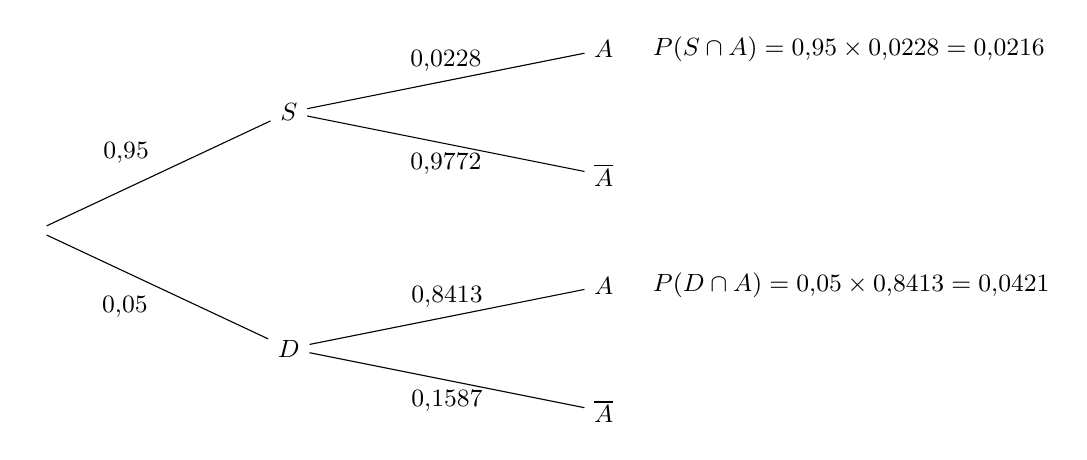
\begin{tikzpicture}[x=1cm,y=1cm,font=\small]
  \node (R) at (0,0) {};
  \node (S) at (3.2,1.5) {$S$};  \node (D) at (3.2,-1.5) {$D$};
  \node (SA) at (7.2,2.3) {$A$}; \node (SN) at (7.2,0.7) {$\overline{A}$};
  \node (DA) at (7.2,-0.7) {$A$}; \node (DN) at (7.2,-2.3) {$\overline{A}$};
  \draw (R) -- (S) node[midway, above left] {$0{,}95$};
  \draw (R) -- (D) node[midway, below left] {$0{,}05$};
  \draw (S) -- (SA) node[midway, above] {$0{,}0228$};
  \draw (S) -- (SN) node[midway, below] {$0{,}9772$};
  \draw (D) -- (DA) node[midway, above] {$0{,}8413$};
  \draw (D) -- (DN) node[midway, below] {$0{,}1587$};
  \node[anchor=west] at (7.7,2.3) {$P(S \cap A) = 0{,}95 \times 0{,}0228 = 0{,}0216$};
  \node[anchor=west] at (7.7,-0.7) {$P(D \cap A) = 0{,}05 \times 0{,}8413 = 0{,}0421$};
\end{tikzpicture}
\end{center}
Probabilités totales ($S$ et $D$ forment une partition)~:
\[ P(A) = P(S)\,P_S(A) + P(D)\,P_D(A) = 0{,}95 \times 0{,}0228 + 0{,}05 \times 0{,}8413 \approx 0{,}0637. \]
La probabilité qu'un palier tiré au hasard déclenche l'alarme est d'environ $6{,}4\,\%$.
\bareme{arbre complet et correct (pondérations $0{,}95$ et $0{,}05$, branches $\alpha$ et $1-\beta$) $0{,}75$~; formule des probabilités totales et résultat $0{,}75$.}
\piege{mettre $\beta = 0{,}1587$ sur la branche $D \to A$~; oublier de pondérer par $0{,}95$ et $0{,}05$~; additionner $0{,}0228 + 0{,}8413$.}
\end{correction}

\begin{correction}[-- Question 3]
\source{\TD, P6 Q2, p.~14 (proportion d'un état parmi les pièces rejetées, même méthode)~; P2 Q3, p.~4 (probabilité conditionnelle inversée)}
On cherche $P_A(D)$~:
\[ P_A(D) = \frac{P(A \cap D)}{P(A)} = \frac{0{,}05 \times 0{,}8413}{0{,}0637} = \frac{0{,}0421}{0{,}0637} \approx 0{,}6606. \]
Avec les valeurs intermédiaires arrondies à $10^{-4}$, on trouve $0{,}6601$~: accepté.\\
Interprétation~: quand l'alarme se déclenche, le palier est réellement défectueux dans environ $2$ cas sur $3$~; un tiers des alarmes sont de \textbf{fausses alarmes}, bien que $\alpha$ soit faible ($2{,}3\,\%$), parce que les paliers sains sont très majoritaires ($95\,\%$).
\bareme{définition de $P_A(D)$ par le quotient $0{,}5$~; calcul $0{,}5$~; interprétation (deux sur trois, rôle des $95\,\%$) $0{,}5$.}
\piege{répondre $P_D(A) = 0{,}8413$ (confusion entre $P_A(D)$ et $P_D(A)$)~; diviser par $P(D) = 0{,}05$ au lieu de $P(A)$.}
\end{correction}

\begin{correction}[-- Question 4]
\source{\TD, P6 Q3, p.~15 (seuil pour $\beta \leq 0{,}5\,\%$, tableau récapitulatif et commentaire)}
a) L'exigence s'écrit $\beta = P_D(\overline{A}) = P_D(V \leq s) \leq 0{,}05$, avec $V \sim \mathcal{N}(4{,}0\,;1{,}0)$. À la limite,
\[ \frac{s - 4}{1} = \texttt{FracNormale}(0{,}05) \approx -1{,}6449 \quad\Longrightarrow\quad s = 4 - 1{,}6449 = 2{,}3551. \]
$\beta$ augmente avec $s$~: il faut $s \leq 2{,}3551$, valeur \textbf{maximale}. On arrondit \textbf{par défaut}~: $s = 2{,}35$ mm/s.\\
Vérification~: $\beta(2{,}35) = 0{,}0495$, exigence respectée~; $\beta(2{,}36) = 0{,}0505$ (arrondi au plus proche), exigence non respectée.\\[4pt]
b) Pour $s = 2{,}35$, avec la loi du palier sain $\mathcal{N}(2{,}0\,;0{,}5)$~:
\[ \alpha = P_S(V > 2{,}35) = 1 - \Phi\!\left(\frac{2{,}35 - 2}{0{,}5}\right) = 1 - \Phi(0{,}7) = 0{,}2420. \]
Commentaire~: en abaissant le seuil de $3{,}0$ à $2{,}35$ mm/s, la non-détection passe de $15{,}9\,\%$ à $4{,}9\,\%$, mais les fausses alarmes passent de $2{,}3\,\%$ à $24{,}2\,\%$~: environ un palier sain sur quatre déclenche l'alarme. Les deux populations se recouvrent~: on ne peut pas réduire $\beta$ sans augmenter $\alpha$. Le choix du seuil est un compromis entre le coût d'un défaut non détecté et celui d'une intervention inutile.
\bareme{a) traduction de l'exigence $0{,}5$~; calcul de $s$ avec le bon $z$ $0{,}5$~; arrondi par défaut justifié $0{,}5$~; b) $\alpha$ $0{,}5$~; commentaire chiffré du compromis $0{,}5$. Si $s$ est faux mais utilisé de façon cohérente en b), ne pas pénaliser deux fois.}
\piege{arrondir à $2{,}36$~; prendre $z = +1{,}6449$ ($s = 5{,}64$)~; utiliser la loi du palier sain pour chercher $s$~; en b), donner $\Phi(0{,}7) = 0{,}7580$ (aire du mauvais côté).}
\par\smallskip{\footnotesize\color{uimmgray}\textbf{Pour aller plus loin (hors barème).} Avec $s = 2{,}35$, la probabilité qu'une alarme soit justifiée tombe à $P_A(D) \approx 0{,}1713$, soit environ une alarme sur six~: à comparer au $0{,}6606$ de la question 3. Les valeurs de l'énoncé sont fictives et ne correspondent à aucun seuil normatif.}
\end{correction}

\end{document}
